\documentclass[12pt]{article}
\usepackage{hyperref}
\usepackage{amsmath}
\usepackage{amsfonts}
\usepackage{amssymb}
\usepackage{graphicx}
\usepackage{caption}

\title{\Huge\textbf{CS215 Assignment 2}}
\author{\Large\textbf{ Group Members :} \\ \\ 
    \large B.Abhinav  23B1018 \\ \\ 
    \large G.Abhiram  23B1084 \\ \\
    \large Sai Likhith 23B1058 
} 
\date{\today}

\begin{document}
\pagenumbering{arabic}
\maketitle
\newpage

\tableofcontents
\newpage

%%%%%%%%%%%%%%%%%%%%%%%% Question 1 %%%%%%%%%%%%%%%%%%%%%%
\section{Mathemagic}
\subsection{Task A}
\textbf{Solution: } \newline
Lets derive the PGF for $X \sim \text{Ber}(p)$. PMF for Ber(p) is given by :
\[P(X=1) = p\]
\[P(X=0) = 1-p\]
G(z) for Bernoulli random variable is given by:

\[G_{Ber}\ =\ E(z^X)\ =\ \sum_{n=0}^{1}P[X\ =\ n]z^n \]

\begin{equation}
    G_{Ber}\ =\ (1-p)z^0+pz^1\ =\ 1-p+pz
\end{equation}

\subsection{Task B}
\textbf{Solution: } \newline
PMF of Bin(n, p) is given by: 
\[P(X=k)\ =\ \binom{n}{k}p^k(1-p)^{n-k}\]
G(z) for Binomial random variable is given by:

\[G_{Bin}\ =\ \sum_{k=0}^nP[X\ =\ k]z^k\]
\[G_{Bin}\ =\ \sum_{k=0}^n\binom{n}{k}(zp)^k(1-p)^{n-k}\]
Using Binomial Theorem :
\[G_{Bin}\ =\ (1-p+zp)^{n}\]
From $G_{Ber}$ in Task A:
\begin{equation}
    G_{Bin}\ =\ G_{Ber}(z)^n
\end{equation}

\subsection{Task C}
\textbf{Solution: } \newline
$X_1,X_2,X_3,\dots,X_k$ are independent non-negative-integer-valued random variables, each distributed with the same probability mass function P and have a common PGF G.
\[X\ =\ X_1+X_2+X_3+\dots+X_k\]
PGF of X is given by :
\[G_{\Sigma}\ =\ E(z^X)\ =\ E(z^{X_1+X_2+X_3+\dots+X_k})\]
\[G_{\Sigma}\ =\ E(z^{X_1}z^{X_2}z^{X_3}\dots z^{X_k})\]
Using the fact that when a, b are 2 independent random variables we have:
\begin{equation}
    E(f(a)g(b))\ =\ E(f(a))E(g(b))
\end{equation}
The proof is as follows:
\[E(f(a)g(b))\ =\ \sum_{a_i\in S(a)}^{}\sum_{b_j\in S(b)}^{}P_a[a=a_i]P_b[b=b_j]a_ib_j\]
As they are independent ie a,P(a) do not depend on b we get:
\[E(f(a)g(b))\ =\ \sum_{a_i\in S(a)}^{}P_a[a=a_i]a_i\sum_{b_j\in S(b)}^{}P_b[b=b_j]b_j\]
This proves the result.
As all $X_i$ are independent we have :

\[G_{\Sigma}\ =\ E(z^{X_1})E(z^{X_2})E(z^{X_3})\dots E(z^{X_k})\]
As all of them have common PGF G we get:
\begin{equation}
    G_{\Sigma}\ =\ G(z)^k
\end{equation}

\subsection{Task D}
\textbf{Solution: } \newline
PMF of Geo(p) is as follows:
\[P[X\ =\ n]\ =\ (1-p)^{n-1}p\]
where X = {1, 2, 3....} . PGF of Geo(p) is :
\[\sum_{n=1}^{\infty}P[X=n]z^n\ =\ \sum_{n=1}^{\infty}(1-p)^{n-1}pz^n\]
\[G_{Geo}\ =\ \frac{p}{1-p}\sum_{n=1}^{\infty}(z(1-p))^n\]
This summation only converges when:
\begin{equation}
    |z(1-p)|<1 \Rightarrow |z|<\frac{1}{|1-p|}
\end{equation}
Using the formula for sum of infinite GP:
\[G_{Geo}\ =\ \frac{p}{1-p}\times\frac{z(1-p)}{1-z(1-p)}\]
under the condition (5) Simplifies to:
\begin{equation}
    G_{Geo}\ =\ \frac{zp}{1-z+zp}
\end{equation}

\subsection{Task E}
\textbf{Solution: } \newline
Consider $X \sim \text{Bin}(n, p)$ and $Y \sim \text{NegBin}(n, p)$ .\\
Let us compute the PGF for Y using the result (4) from Task C. We know that NegBin(n, p) random variable can be written as sum of n independent Geo(p) random variables.
\[G_{Y}^{(n,p^{-1})}(z^{-1})\ =\ G_{Geo}^{p^{-1}}(z^{-1})^{n}\]
Using (6) with p and z replaced with $p^{-1}$ and $z^{-1}$ We ge :
\[G_{Y}^{(n,p^{-1})}(z^{-1})\ =\ \left(\frac{z^{-1}p^{-1}}{1-z^{-1}+z^{-1}p^{-1}}\right)^{n}\]
This simplifies to:
\[G_{Y}^{(n,p^{-1})}(z^{-1})\ =\ \left(\frac{1}{1-p+zp}\right)^{n}\]
Inverse on both sides and using (2):
\[\left(G_{Y}^{(n,p^{-1})}(z^{-1})\right)^{-1}\ =\ (1-p+zp)^n\ =\ G_{X}^{(n,p)}(z)\]
Replacing p with $p^{-1}$ and $z^{-1}$ we prove the result and inverting:
\begin{equation}
    G_{Y}^{(n,p)}(z)\ =\ \left(G_{X}^{(n,p^{-1})}(z^{-1})\right)^{-1}
\end{equation}

\subsection{Task F}
\textbf{Solution: } \newline
PMF of $Y \sim \text{NegBin}(n, p)$ is given by(for k = n, n+1, $\dots$):
\begin{equation}
    P[Y\ =\ k]\ =\ \binom{k-1}{n-1}p^n(1-p)^{k-n}
\end{equation}
The RHS of the equation (7) simplifies to:
\[(1-p^{-1}+z^{-1}p^{-1})^{-n}\ =\ \left(\frac{p^{n}z^{n}}{(1-z+pz)^n}\right)\]
The PGF of NegBin(n, p) by definition was:
\[G_Y^{(n,p)}\ =\ E(z^Y)\ =\ \sum_{k=n}^{\infty}\binom{k-1}{n-1}p^n(1-p)^{k-n}z^k\]
Equate both of them and use k = n + r on LHS:
\[\sum_{r=0}^{\infty}\binom{n+r-1}{n-1}p^n(1-p)^{r}z^{r+n}\ =\ \frac{p^{n}z^{n}}{(1-z+pz)^n}\]
Cancelling the common terms this simplifies to:
\[(1-z(1-p))^{-n}\ =\ \sum_{r=0}^{\infty}\binom{n+r-1}{n-1}(z(1-p))^{r}\]
We have proved in (5) that PGF for Y is only defined under $|z(1-p)<1$. \\
Substitute x = z(1-p) under $|x|<1$ to get:
\[(1-x)^{-n}\ =\ \sum_{r=0}^{\infty}\binom{n+r-1}{n-1}x^r \]
Using \[\binom{n}{r} = \binom{n}{n-r}\] and substituting x with -x we get:
\begin{equation}
    (1+x)^{-n}\ =\ \sum_{r=0}^{\infty}(-1)^{r}\binom{n+r-1}{r}x^r
\end{equation}
From the general definition of $\binom{n}{r}$ we have:
\[\binom{-n}{r}\ =\ \frac{(-n)(-n-1)(-n-2)....(-n-r+1)}{r!}\]
\[\binom{-n}{r}\ =\ (-1)^{r}\frac{(n+r-1)(n+r-2)...(n+1)(n)}{r!}\]
\[\binom{-n}{r}\ =\ (-1)^{r}\binom{n+r-1}{r}\]
Using this in (9) we get \\
For $n\in N$ and $|x|<1$ :
\begin{equation}
    (1+x)^{-n}\ =\ \sum_{r=0}^{\infty}(-1)^{r}\binom{n+r-1}{r}x^r\ =\ \sum_{r=0}^{\infty}\binom{-n}{r}x^r
\end{equation}
that is the Binomial Theorem for negative exponent.

\subsection{Task G}
\textbf{Solution: } \newline
We have for a random variable X with PGF G(z)
\[G(z)\ =\ \sum_{n=0}^{\infty}P[X=n]z^n\]
\[G'(z)\ =\ \sum_{n=0}^{\infty}nz^{n-1}P[X=n]\]
Substituting z = 1 we get:
\begin{equation}
    E(X)\ =\ \sum_{n=0}^{\infty}nP[X=n]\ =\ G'(1)
\end{equation}
Mean for Bern(p):
\[E_{Ber}\ =\ G'_{Ber}(1),\ G_{Ber}(z)=1-p+zp \Rightarrow G'_{Ber}(z)=p \]
Hence :
\begin{equation}
    E_{Ber}\ =\ p
\end{equation}
Mean for Bin(n, p)
\[G_{Bin}(z)\ =\ (1-p+zp)^n \Rightarrow G'_{Bin}(z)=np(1-p+zp)^{n-1} \Rightarrow G'_{Bin}(1)=np\]
Hence 
\begin{equation}
    E_{Bin}\ =\ np
\end{equation}
Mean for Geo(p)
\[G_{Geo}(z)\ =\ \frac{zp}{1-z+zp} \Rightarrow G'_{Geo}(z)=\frac{(1-z+zp)(p)-(zp)(p-1)}{(1-z+zp)^2}\]
\[G'_{Geo}(z)\ =\ \frac{p}{(1-z+zp)^2} \Rightarrow G'_{Geo}(1)=\frac{1}{p}\]
Hence
\begin{equation}
    E_{Geo}(z)\ =\ \frac{1}{p}
\end{equation}
Mean for NegBin(n, p)
\[G_{NegBin}(z)\ =\ G_{Geo}(z)^{n} \Rightarrow G'_{NegBin}(z)=nG_{Geo}(z)^{n-1}G'_{Geo}(z)\]
\[G'_{NegBin}(1)\ =\ \frac{n}{p}\]
Hence 
\[E_{NegBin} =\ \frac{n}{p}\]

%%%%%%%%%%%%%%%%%%%%%%%%%%%%%%%%%%%%%%%%%%%%%%%%%%%%%%%%%%%%%%

\section{Normal Sampling}
\subsection{Task A}
\textbf{Solution: } \newline
It suffices to prove that $f_{Y}(y)=1$,
Let us prove the following theorem first: \\
Given random variables $X$ and $Y$ with PDFs $f_X(x)$ and $f_Y(y)$, under an invertible transformation $Y = g(X)$, 
\[
f_Y(y) = \frac{f_X(g^{-1}(y))}{\left| g'(g^{-1}(y)) \right|}
\]
\textbf{Proof:} \\
Let $x_1, x_2, y_1, y_2 \in \mathbb{R}$ such that $y_1 = g(x_1)$ and $y_2 = g(x_2)$.
We have we have assuming g is non decreasing::
\[
P(x_1 \leq X \leq x_2) = P(y1 \leq Y \leq y2)
\]
since $g$ is invertible.
The probability of the event must be the same whether expressed in terms of $X$ or $Y$. This can be written as:
\[
\int_{x_1}^{x_2} f_X(x) \, dx = \int_{y_1}^{y_2} f_Y(y) \, dy
\]
Using the transformation $y = g(x)$, we know that:
\[
x=g^{-1}(y)\ and\ dx=(g^{-1})'(y)dy
\]
Thus, the integral becomes:
\[
\int_{y_1}^{y_2} f_Y(y) \, dy = \int_{y_1}^{y_2} f_X(g^{-1}(y))(g^{-1})'(y)dy
\]
As the above is true $\forall y1,y2 \in R$, The integrands must be equal.This can also be shown by treating them as functions and differentiating both integrals.(Second Fundamental Theorem of Calculus)
\[
f_Y(y) \ =\ f_X(g^{-1}(y)) \cdot (g^{-1})'(y)
\]
From calculus we have $(g^{-1})'(y)=\frac{1}{g'(g^{-1}(y))}$. It follows that:

\[
\boxed{f_Y(y) = \frac{f_X(g^{-1}(y))}{\left| g'(g^{-1}(y)) \right|}}
\]
The modulus is accounting for the case when g is non increasing as PDF's are always non negative.
Coming back to our question the invertible transformation $g$ is $F_{X}$ the CDF of X.
\[g(x)=\int_{-\infty}^{x}f_{X}(x)dx\  \Rightarrow\ g'(x)=f_{X}(x) \] 
Therefore here we have $g'(g^{-1}(y))=f_{X}(g^{-1}(y))$ and $g'\ge 0$ as CDF is non decreasing we have :
\[f_{Y}(y)=1\]
Therefore we proved that $Y$ is uniformly distributed in $[0,1]$.

\subsection{Task B}
From the theorem we have proved in Task A we can sample a standard normal distribution.
Let X be a standard normal disrtribution. We have
\[f_X(x) = \frac{1}{\sqrt{2\pi}} e^{-\frac{x^2}{2}}\]
Since $F_{X}'(x)=f(x) > 0\ \ ,F_{X}(x)$ is invertible.
We know that $Y=F_{X}(X)$ is a uniform distribution in [0,1] from Task A.\\
Our algorithm $\mathcal{A}$ invloves computing the inverse $G_{X}(Y)$ of $F_{X}(X)$ and then mapping the uniform distribution $Y$ using it.\\
Using this we can sample a standard normal distribution from a uniform distribution Y in [0,1].\\
This also implies that $\forall u \in R$ we have 
\[F_{\mathcal{A}}(u)=F_{X}(u)\ and\ f_{\mathcal{A}}(u)=f_{X}(u)\]

\subsection{Task C}
\textbf{Check the code in 2c.py}
\begin{minipage}{\linewidth}
    \begin{center}
        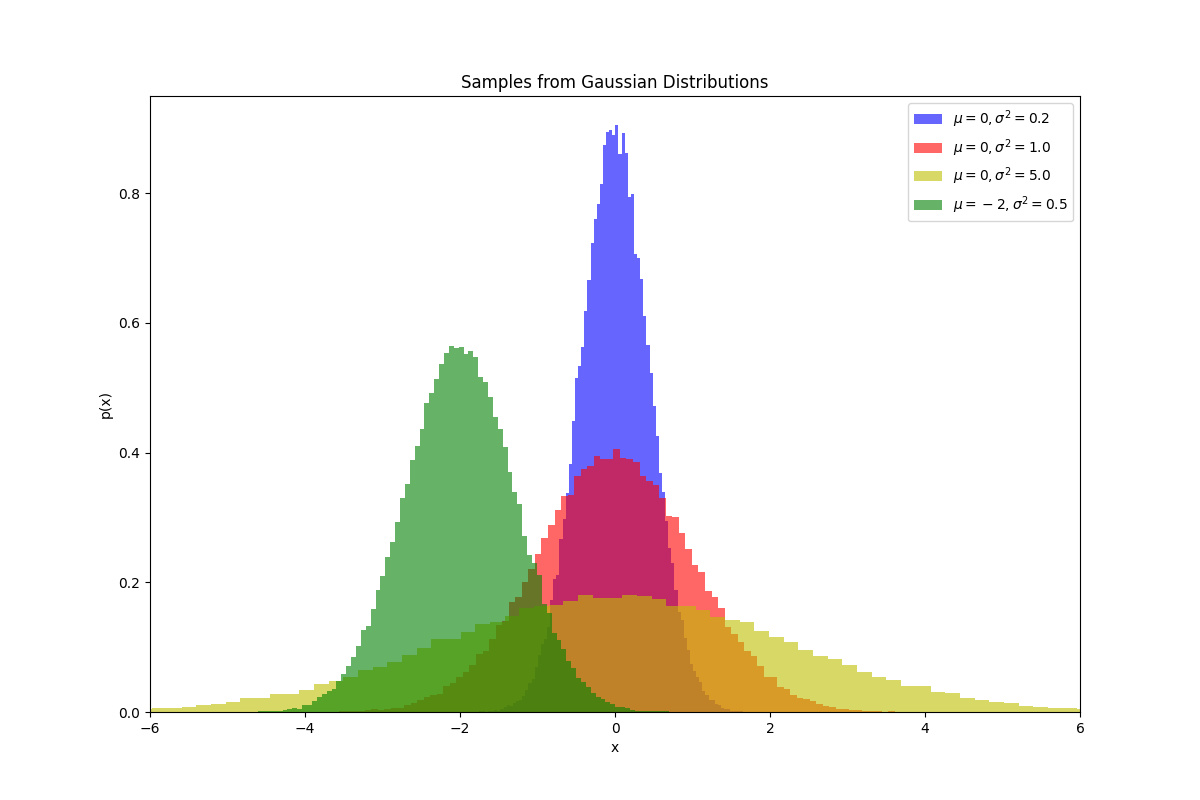
\includegraphics[width=0.5\textwidth]{images/2c.png}
        \captionof{figure}{The Bell curve}
    \end{center}
\end{minipage}

\subsection{Task D}
\textbf{Check the code in 2d.py} \\
The shape of the graph, which appears to be approximately bell-shaped for large depth(h), suggests that the distribution of the final positions of the balls is approximately normal.
\newline
This is because :
\begin{enumerate}
    \item The majority of the balls tend to fall in the middle pockets.
    \item The number of balls in each pocket decreases as you move away from the middle.
    \item The distribution is symmetric around the middle.
\end{enumerate}
\begin{minipage}{\linewidth}
    \begin{center}
        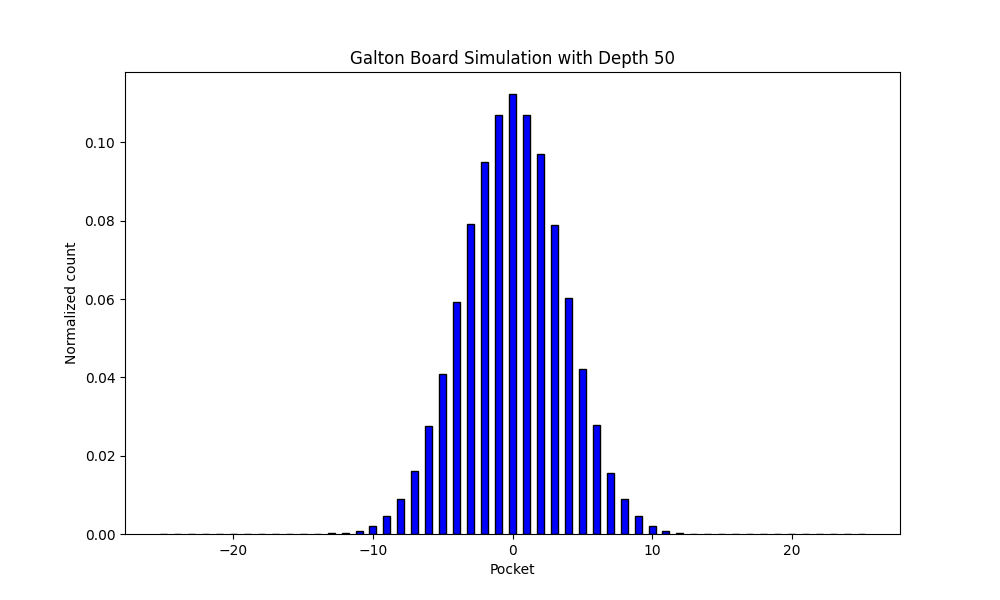
\includegraphics[width=0.5\textwidth]{images/2d2.png}
        \captionof{figure}{Plot for h = 50 and N = 100000}
    \end{center}
\end{minipage}
\begin{minipage}{\linewidth}
    \begin{center}
        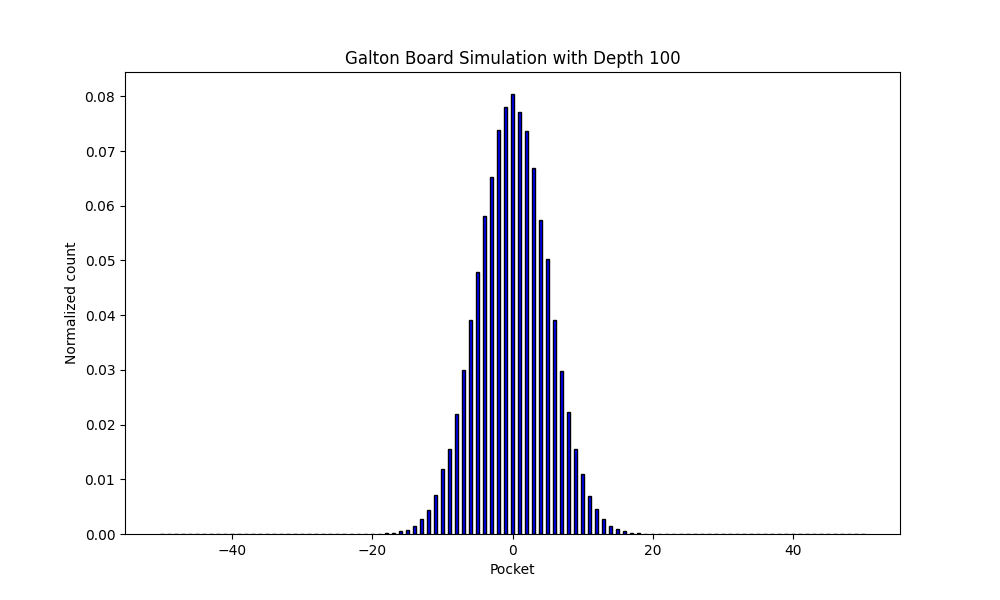
\includegraphics[width=0.5\textwidth]{images/2d3.png}
        \captionof{figure}{Plot for h = 100 and N = 100000}
    \end{center}
\end{minipage}

\section{Fitting Data}
\subsection{Task A}


\end{document}
